% Provenance (never printed): see sources/outline_sources.md (Year 2: effusive and explosive
% eruptions, eruptive styles, eruption columns, pyroclastic deposits, explosivity index,
% volcano monitoring).
% Curves from figdata/bachelor-2/eruptions.py (closed-system gas fraction, Cotopaxi Layer 5
% thinning, GVP frequency-size law, column height fits, Mogi uplift); exercise and problem
% values in the Book 4 scratch calculators calc/ch06.py and calc/ch06pb.py.
\chapter{Éruptions volcaniques}\label{ch:b2:eruptive-styles}

Le 15 juin 1991, le mont Pinatubo, aux Philippines, a projeté plus de cinq
kilomètres cubes de matériaux~; son nuage de cendres s'est élevé jusqu'à
\qty{35}{km}, le sommet s'est effondré en une \omterm{def:b2:eruptive-styles:caldera}{caldeira} large de \qty{2.5}{km}, et les
vingt millions de tonnes de dioxyde de soufre injectées dans la stratosphère ont refroidi le
globe entier d'environ un demi-degré pendant deux ans. Une semaine plus tôt, le premier
\omterm{def:b2:magma-emplacement:magma}{magma} parvenu à la surface n'avait rien fait de tel~: ayant perdu l'essentiel de son
gaz pendant la remontée, il avait suinté en un \omterm{def:b2:eruptive-styles:dome}{dôme de lave}. Sur le Kīlauea, à Hawaï,
l'éruption du Pu`u~`\=O`\=o a répandu \qty{4.4}{km^3} de lave, un volume comparable,
en trente-cinq ans, sous forme de fontaines et de coulées qui ont détruit 215 bâtiments
sans jamais élever de haute colonne de cendres. Même Terre, mêmes lois, trois comportements~: ce qui les distingue
est la quantité de gaz qu'un \omterm{def:b2:magma-emplacement:magma}{magma} transporte, la capacité de ce gaz à quitter
discrètement le liquide, et la vitesse de remontée du \omterm{def:b2:magma-emplacement:magma}{magma}. Ce chapitre suit une éruption
depuis les bulles du conduit jusqu'à la colonne au-dessus de l'évent et aux dépôts qu'elle
laisse, puis mesure les éruptions, les compte et surveille les volcans pour y déceler
les signes d'une éruption imminente.
% ledger: usgs:pinatubo-1991, usgs:puuoo

\begin{recall}
\textbf{Des volumes scolaires}~: un volcan, son évent et son cratère, la chambre
magmatique située dessous, la lave et les cendres volcaniques. \textbf{Du
\cref{ch:b2:magma-emplacement}}~: les \omterm{def:b2:magma-emplacement:volatiles}{volatils magmatiques}, leur exsolution sous la
\omterm{def:b2:magma-emplacement:volatiles}{pression de saturation en volatils}, la loi de solubilité de l'eau en racine carrée $w = s\sqrt p$ avec
$s \approx 0.34$ pour cent par $\sqrt{\unit{MPa}}$ pour le basalte et $0.44$ pour
la rhyolite, et les viscosités des liquides, séparées de dix ordres de grandeur.
\textbf{Des volumes de physique}~: la loi des gaz parfaits $pV = nRT$~; la poussée
d'Archimède~; l'analyse dimensionnelle, qui construit l'unique combinaison des grandeurs données
qui a la dimension du résultat~; la portée d'un projectile, $v^2\sin 2\theta/g$
sans résistance de l'air. \textbf{Des volumes de mathématiques}~: le processus de Poisson,
dans lequel des événements indépendants à taux constant $\lambda$ donnent au moins un événement
dans un temps $t$ avec la probabilité $1 - e^{-\lambda t}$~; les droites des moindres carrés.
Du volume de première année~: les séismes et leurs magnitudes.
\end{recall}

\section{Effusif ou explosif}

\begin{definition}[Éruptions effusives et explosives, fragmentation]\label{def:b2:eruptive-styles:regimes}
Une \emph{éruption effusive}\index{éruption effusive} est dominée par
l'émission de lave, qui s'écoule loin de l'évent comme un liquide cohérent. Une
\emph{éruption explosive}\index{éruption explosive} produit surtout des fragments,
des cendres, de la ponce et des débris balistiques, transportés par un gaz en expansion. La
\emph{fragmentation du magma}\index{fragmentation du magma} est la rupture d'un liquide continu
contenant des bulles en un gaz continu qui emporte des gouttes et des fragments de liquide~;
elle transforme un écoulement effusif en éruption explosive.
\end{definition}
% ledger: usgs:glossary-ch6, cassidy18:fragmentation

Ce qui commande la transition, c'est le gaz. Un \omterm{def:b2:magma-emplacement:magma}{magma} qui remonte des profondeurs transporte
de l'eau et du dioxyde de carbone dissous~; en dessous de sa \omterm{def:b2:magma-emplacement:volatiles}{pression de saturation en volatils}, ils
sortent de la solution sous forme de bulles, qui grossissent à mesure que la pression baisse.
Si elles restent dans le liquide, le gaz occupe vite l'essentiel du volume.

\begin{proposition}[Fraction volumique de gaz lors d'un dégazage en système fermé]\label{prop:b2:eruptive-styles:gas}
Soit un \omterm{def:b2:magma-emplacement:magma}{magma} contenant une fraction massique $w_0$ d'eau, de solubilité $w(p) =
s\sqrt p$, et supposons que l'eau exsolvée reste avec le liquide sous forme de gaz parfait
à la température $T$. Sous la \omterm{def:b2:magma-emplacement:volatiles}{pression de saturation en volatils} $p_s = (w_0/s)^2$, un kilogramme de
\omterm{def:b2:magma-emplacement:magma}{magma} renferme $x = w_0 - s\sqrt p$ kilogramme de vapeur, et la fraction volumique
de gaz est
\[
\phi(p) = \frac{V_g}{V_g + V_m}, \qquad V_g = \frac{x\,RT}{M p}, \qquad
V_m = \frac{1 - x}{\rho_m},
\]
où $M = \qty{0.018}{kg/mol}$ est la masse molaire de l'eau et $\rho_m$ la masse volumique
du \omterm{def:b2:magma-emplacement:magma}{liquide silicaté}.
\end{proposition}

\begin{proof}
Au-dessus de $p_s$, le liquide peut retenir toute son eau, et aucun gaz n'existe. En dessous de $p_s$, le
liquide ne conserve que sa solubilité $s\sqrt p$~; une masse $x = w_0 - s\sqrt p$ par
kilogramme de \omterm{def:b2:magma-emplacement:magma}{magma} est donc de la vapeur. Cette vapeur, soit $x/M$ moles, occupe $xRT/(Mp)$ selon
la loi des gaz parfaits~; les $1 - x$ kilogrammes de liquide restant occupent $(1 - x)/\rho_m$.
La fraction volumique en découle.
\end{proof}
% ledger: moore98:h2o

Comme $V_g$ croît comme $1/p$, la mousse gonfle le plus vite près de la surface. La
figure ci-dessous suit une rhyolite à \qty{5}{\percent} d'eau et un basalte
à \qty{1}{\percent}. La rhyolite sature à \qty{127}{MPa}, soit environ
\qty{5}{km} de profondeur~; à \qty{10}{MPa}, son gaz occupe déjà \qty{82}{\percent} du
volume. Dans un modèle publié de l'écoulement dans le conduit, le \omterm{def:b2:magma-emplacement:magma}{magma} se fragmente lorsque le
gaz occupe \qty{85}{\percent} de son volume, un niveau que cette rhyolite atteint à
\qty{8.2}{MPa}, soit environ \qty{330}{m} sous l'évent pour un gradient de pression de
\qty{0.025}{MPa/m}. Le basalte ne sature qu'à \qty{8.7}{MPa} et atteint la même
mousse à \qty{1.8}{MPa}, à moins de cent mètres de la surface.
% ledger: cassidy18:fragmentation, cassidy18:ascent

\begin{omfigure}
\centering
\begin{tikzpicture}
\begin{axis}[omrecord, width=0.82\linewidth, height=5.6cm, xmode=log,
  xmin=0.01, xmax=200, ymin=0, ymax=1,
  xlabel={pression (\unit{MPa})}, ylabel={fraction volumique de gaz $\phi$},
  legend pos=south west, legend style={font=\scriptsize},
  tick label style={font=\scriptsize}, label style={font=\small}]
\addplot[very thick, red!70!black] table[x=p_MPa, y=rhyolite] {figdata/out/bachelor-2-eruptions-gas.dat};
\addlegendentry{rhyolite, \qty{5}{\percent} H$_2$O, \qty{850}{\celsius}}
\addplot[very thick, black, dashed] table[x=p_MPa, y=basalt] {figdata/out/bachelor-2-eruptions-gas.dat};
\addlegendentry{basalte, \qty{1}{\percent} H$_2$O, \qty{1200}{\celsius}}
\draw[densely dotted, thick, gray] (axis cs:0.01,0.85) -- (axis cs:200,0.85);
\node[anchor=north west, font=\scriptsize, inner sep=1pt] at (axis cs:0.012,0.835) {fragmentation dans un modèle de conduit};
\end{axis}
\end{tikzpicture}
\par\smallskip{\small Fraction volumique de vapeur d'eau exsolvée en fonction de la pression
lors d'un dégazage en système fermé (\cref{prop:b2:eruptive-styles:gas}), avec les lois de
solubilité du \cref{ch:b2:magma-emplacement}. La pression diminue vers la gauche, à mesure que le
\omterm{def:b2:magma-emplacement:magma}{magma} remonte~; le trait pointillé marque la fraction de gaz à laquelle un modèle publié de conduit
fragmente le \omterm{def:b2:magma-emplacement:magma}{magma}.}
\end{omfigure}
% ledger: moore98:h2o, cassidy18:fragmentation

Un basalte se fragmenterait donc lui aussi s'il gardait son gaz, et c'est bien ce qui se passe
dans une fontaine de lave hawaïenne, près de l'évent. Ce qui rend la plupart des éruptions basaltiques
douces, c'est que le gaz ne reste pas. Dans un \omterm{def:b2:magma-emplacement:magma}{liquide silicaté} peu visqueux, les bulles remontent
à travers le liquide, fusionnent et s'échappent~; une fois connectées en un réseau perméable,
ce qui se produit pour des fractions de gaz comprises entre \qty{30}{\percent} et \qty{78}{\percent}
dans les expériences, le gaz fuit à travers les parois et l'évent sans entraîner le
liquide~: le \omterm{def:b2:magma-emplacement:magma}{magma} se dégaze en système ouvert et atteint la surface sous forme de
lave. Un \omterm{def:b2:magma-emplacement:magma}{magma} visqueux conserve au contraire ses bulles et se fragmente, le liquide se brisant
comme du verre lorsqu'on l'étire plus vite qu'il ne peut s'écouler. La vitesse de remontée décide
entre les deux autant que la composition~: sur de nombreuses éruptions, l'activité effusive
va de pair avec des vitesses de décompression voisines de \qty{0.0001}{MPa/s}, et les \omterm{def:b2:eruptive-styles:regimes}{éruptions explosives}
avec des vitesses voisines de \qty{1}{MPa/s}~; un changement de viscosité du liquide
de l'ordre d'une demi-unité logarithmique, soit un facteur trois environ, peut faire basculer une éruption d'un régime à l'autre.
Le premier \omterm{def:b2:eruptive-styles:dome}{dôme de lave} du Pinatubo et son éruption paroxysmale une semaine plus tard
venaient du même \omterm{def:b2:magma-emplacement:magma}{magma}~: le premier lot avait eu le temps de perdre son gaz, pas le second.
% ledger: cassidy18:fragmentation, cassidy18:ascent, usgs:pinatubo-1991

De l'eau venue de l'extérieur produit l'effet du gaz propre au \omterm{def:b2:magma-emplacement:magma}{magma}. Une nappe souterraine, un lac ou la mer
qui rencontre le \omterm{def:b2:magma-emplacement:magma}{magma} se vaporise en un instant, et la dilatation de l'eau surchauffée
pulvérise le \omterm{def:b2:magma-emplacement:magma}{magma}~: les expériences montrent que plus de \qty{30}{\percent} de la chaleur disponible
peut être convertie en énergie mécanique. Même un \omterm{def:b2:magma-emplacement:magma}{magma} pauvre en gaz peut alors
entrer en \omterm{def:b2:eruptive-styles:regimes}{éruption explosive}.
% ledger: cassidy18:fragmentation

\section{Styles éruptifs}

Les volcanologues nomment les éruptions d'après des exemples classiques. Ces noms décrivent l'aspect
d'une éruption, et ils se fondent les uns dans les autres~; une même éruption passe souvent
par plusieurs styles.

\begin{definition}[Styles éruptifs]\label{def:b2:eruptive-styles:styles}
Par ordre croissant d'explosivité, parmi les éruptions entraînées par le gaz propre du \omterm{def:b2:magma-emplacement:magma}{magma}~:
\begin{itemize}
\item une \emph{éruption hawaïenne}\index{éruption hawaïenne} produit des fontaines de
lave basaltique très fluide, de quelques dizaines à quelques centaines de mètres de haut, alimentant des coulées de lave~;
\item une \emph{éruption strombolienne}\index{éruption strombolienne} est une suite
de brefs jaillissements qui projettent des grumeaux incandescents de \omterm{def:b2:magma-emplacement:magma}{magma}
basaltique à basaltique-andésitique, jusqu'à une centaine de mètres environ,
sans colonne soutenue~;
\item une \emph{éruption vulcanienne}\index{éruption vulcanienne} est une explosion brève et violente
de gaz accumulé sous un bouchon de lave solidifiée, qui brise ce bouchon et projette des blocs
et une colonne sombre de cendres fines, typiquement à partir d'un \omterm{def:b2:magma-emplacement:magma}{magma}
intermédiaire~;
\item une \emph{éruption plinienne}\index{éruption plinienne} est un jet soutenu de gaz
et de \omterm{def:b2:magma-emplacement:magma}{magma} fragmenté, en général silicique, qui alimente une colonne montant dans la
stratosphère pendant des heures à des jours et répand une nappe de ponce et de cendres sur
des milliers de kilomètres carrés.
\end{itemize}
Lorsque de l'eau extérieure entraîne la fragmentation, une \emph{éruption
phréatomagmatique}\index{éruption phréatomagmatique} projette de la vapeur avec des fragments
de \omterm{def:b2:magma-emplacement:magma}{magma} frais, tandis qu'une \emph{éruption phréatique}\index{éruption phréatique} est une
explosion par la vapeur d'une nappe souterraine ou superficielle chauffée par du \omterm{def:b2:magma-emplacement:magma}{magma} ou une roche chaude,
qui projette de la vapeur et des fragments de roches plus anciennes, mais aucun \omterm{def:b2:magma-emplacement:magma}{magma} frais.
\end{definition}
% ledger: nps:styles, usgs:glossary-ch6

Chaque style a ses éruptions types. Le Pu`u~`\=O`\=o, sur le Kīlauea, fut hawaïen pendant
la plupart de ses trente-cinq ans et de ses soixante et un épisodes, avec des fontaines qui s'élevaient
en général à \qtyrange{10}{100}{m} et parfois à plus de \qty{500}{m}. Stromboli, le
« phare de la Méditerranée », a donné son nom aux jaillissements qui construisent les
cônes de scories. Des explosions vulcaniennes ont secoué le Trident, en Alaska, par intermittence entre
1953 et 1974. Le Vésuve, en 79 de notre ère, décrit par Pline le Jeune, a donné son nom aux
\omterm{def:b2:eruptive-styles:styles}{éruptions pliniennes}~; le mont Saint-Helens, le 18~mai~1980, et Novarupta, en 1912, dont
la colonne a dépassé \qty{30}{km} au cours d'une éruption qui a duré près de trois jours, sont
des exemples modernes.
Les cas intermédiaires, à colonnes inférieures à environ \qty{20}{km}, soutenues mais instables,
sont dits sous-pliniens. En présence d'eau, une \omterm{def:b2:eruptive-styles:styles}{éruption strombolienne} devient surtseyenne,
du nom de l'éruption du Surtsey, en 1963, au large de l'Islande, et construit de basses couronnes de
tuf et des maars~; une \omterm{def:b2:eruptive-styles:styles}{éruption plinienne} devient phréatoplinienne. Au Pinatubo, des explosions de vapeur ont fait sauter
trois cratères sur le flanc nord en mars et avril 1991, deux
mois avant l'éruption paroxysmale~: elles étaient phréatiques.
% ledger: nps:styles, usgs:puuoo, usgs:glossary-ch6, usgs:pinatubo-deposits

\begin{definition}[Dôme de lave]\label{def:b2:eruptive-styles:dome}
Un \emph{dôme de lave}\index{dôme de lave} est un monticule à flancs raides de lave visqueuse,
généralement dacitique ou rhyolitique, extrudée lentement d'un évent et s'accumulant au-dessus de lui
au lieu de s'écouler.
\end{definition}
% ledger: usgs:glossary-ch6

Les dômes sont ce que fait un \omterm{def:b2:magma-emplacement:magma}{magma} visqueux lorsqu'il a perdu son gaz~: le premier \omterm{def:b2:magma-emplacement:magma}{magma} du Pinatubo,
en juin 1991, et le dôme qui a grandi dans le cratère du mont Saint-Helens en dix-sept
épisodes entre 1980 et 1986, jusqu'à \qty{267}{m} au-dessus du fond du cratère.
Un dôme peut aussi former le bouchon sous lequel s'accumule la prochaine explosion vulcanienne,
et son effondrement peut libérer la pression sur le \omterm{def:b2:magma-emplacement:magma}{magma} riche en gaz situé dessous. Les
photographies ci-dessous montrent les deux extrêmes de la gamme.
% ledger: usgs:pinatubo-1991, usgs:msh-dome, cassidy18:fragmentation

\begin{omfigure}
\centering
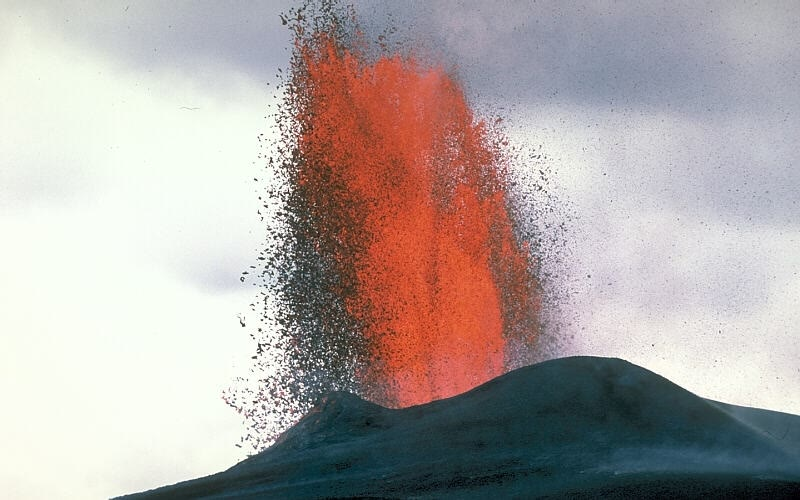
\includegraphics[height=4.3cm]{images/book4/b2-kilauea-fountain.jpg}\hfill
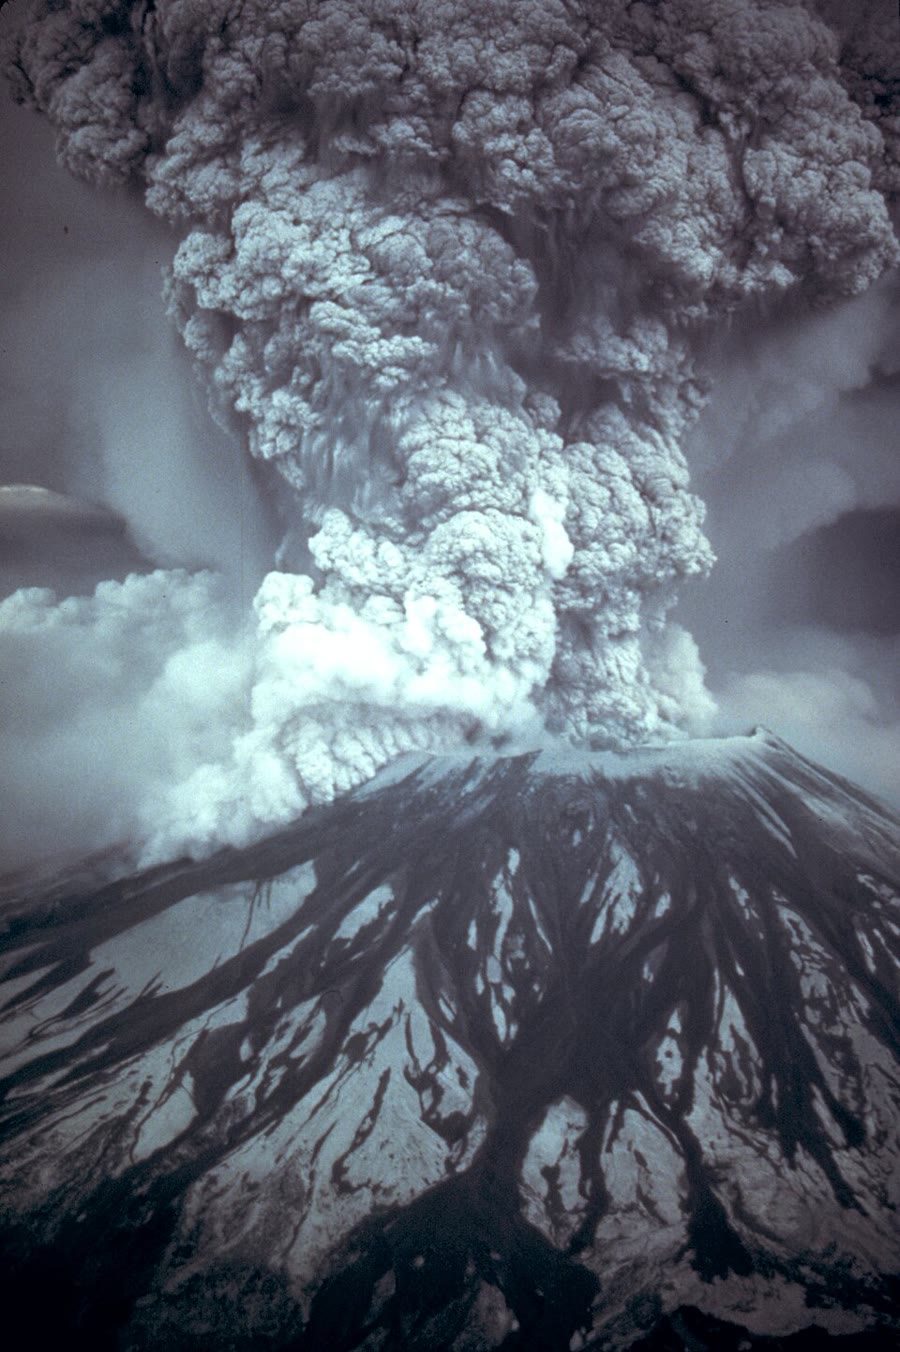
\includegraphics[height=4.3cm]{images/book4/b2-st-helens-column.jpg}\hfill
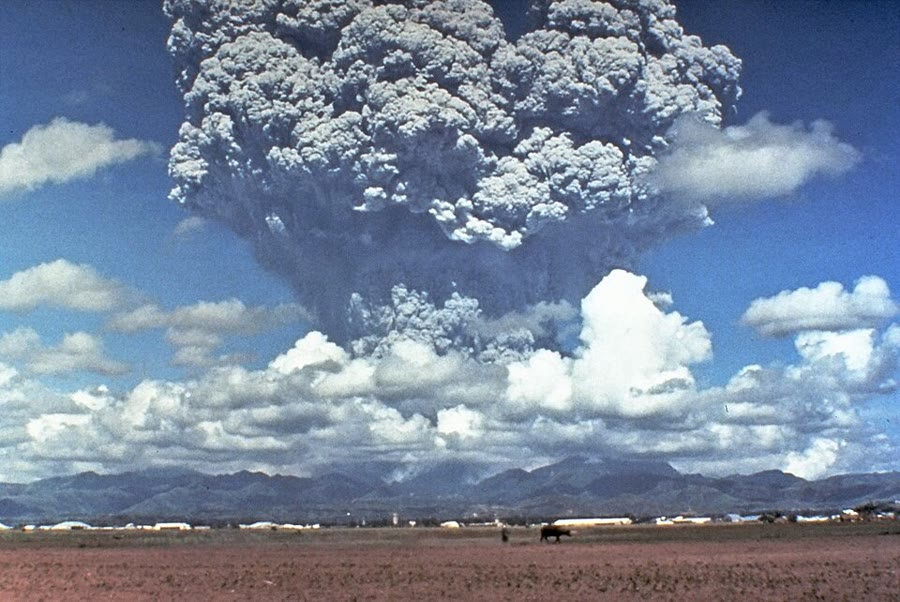
\includegraphics[height=4.3cm]{images/book4/b2-pinatubo-column.jpg}
\par\smallskip{\small À gauche~: une fontaine hawaïenne sur le cône du Pu`u~`\=O`\=o, au Kīlauea,
en octobre 1983 (J.\,D.~Griggs, USGS). Au centre~: la colonne plinienne du mont Saint-Helens,
le 18 mai 1980 (Austin Post, USGS). À droite~: la \omterm{def:b2:eruptive-styles:column}{colonne éruptive} du mont Pinatubo le
12 juin 1991, trois jours avant l'éruption paroxysmale (Dave Harlow, USGS). Les trois
photographies sont dans le domaine public.}
\end{omfigure}
% ledger: usgs:puuoo, usgs:msh-may18, usgs:pinatubo-1991

\section{Colonnes éruptives}

\begin{definition}[Colonne éruptive]\label{def:b2:eruptive-styles:column}
Une \emph{colonne éruptive}\index{colonne éruptive} est la masse ascendante de gaz et de fragments
au-dessus d'un évent explosif. Elle comporte trois parties~: un \emph{jet}, ou
région de poussée des gaz, où le mélange quitte l'évent vite
mais plus dense que l'air, et monte par son élan~; une région \emph{convective},
où le mélange, ayant englouti et réchauffé assez d'air pour devenir plus léger
que son environnement, monte par poussée d'Archimède~; et un \emph{nuage en parapluie}, qui s'étale
latéralement, au niveau où la masse volumique de la colonne égale celle de l'atmosphère.
\end{definition}
% ledger: usgs:glossary-ch6, nps:styles, aubry23:fits

\begin{omfigure}
\centering
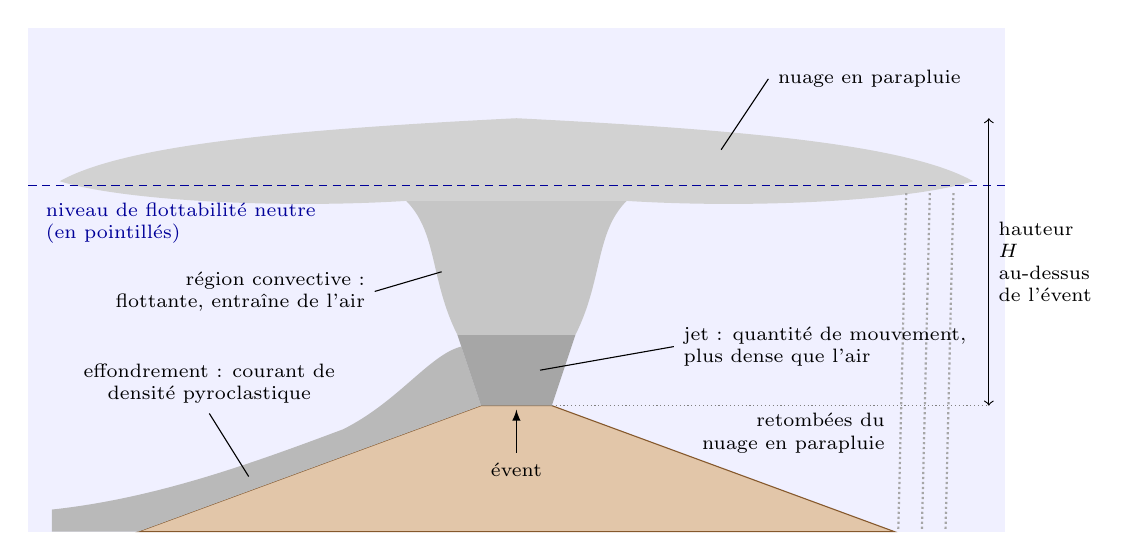
\begin{tikzpicture}[x=1cm, y=1cm, font=\scriptsize]
% atmosphere and ground
\fill[blue!6] (-6.2,0) rectangle (6.2,6.4);
% volcano
\fill[brown!45, draw=brown!70!black] (-4.8,0) -- (-0.45,1.6) -- (0.45,1.6) -- (4.8,0) -- cycle;
% collapse branch (left): a density current hugging the flank
\fill[gray!55] (-0.45,1.6) -- (-0.7,2.35) .. controls (-1.1,2.25) and (-1.5,1.65) .. (-2.2,1.3)
  .. controls (-3.4,0.85) and (-4.6,0.42) .. (-5.9,0.28) -- (-5.9,0) -- (-4.8,0) -- cycle;
% jet
\fill[gray!70] (-0.45,1.6) -- (0.45,1.6) -- (0.75,2.5) -- (-0.75,2.5) -- cycle;
% convective column
\fill[gray!45] (-0.75,2.5) .. controls (-1.1,3.2) and (-1.0,3.8) .. (-1.4,4.2)
  -- (1.4,4.2) .. controls (1.0,3.8) and (1.1,3.2) .. (0.75,2.5) -- cycle;
% umbrella
\fill[gray!35] (-1.4,4.2) .. controls (-3,4.1) and (-5,4.2) .. (-5.8,4.45)
  .. controls (-5,4.9) and (-3,5.1) .. (0,5.25) .. controls (3,5.1) and (5,4.9) .. (5.8,4.45)
  .. controls (5,4.2) and (3,4.1) .. (1.4,4.2) -- cycle;
\draw[densely dashed, blue!60!black] (-6.2,4.4) -- (6.2,4.4);
% fallout from the far end of the umbrella, down to the ground
\foreach \x in {4.95,5.25,5.55} {\draw[gray!70, densely dotted, thick] (\x,4.3) -- (\x-0.1,0.02);}
\draw[gray, densely dotted] (0.45,1.6) -- (6.0,1.6);
\draw[<->] (6.0,1.6) -- (6.0,5.25) node[midway, right, align=left] {hauteur\\$H$\\au-dessus\\de l'évent};
% labels
\node[anchor=north west, align=left, blue!60!black] at (-6.1,4.3) {niveau de flottabilité neutre\\(en pointillés)};
\draw (-0.95,3.3) -- (-1.8,3.05) node[left, align=right] {région convective~:\\flottante, entraîne de l'air};
\draw (0.3,2.05) -- (2.0,2.35) node[right, align=left] {jet~: quantité de mouvement,\\plus dense que l'air};
\draw (2.6,4.85) -- (3.2,5.75) node[right] {nuage en parapluie};
\node[anchor=east, align=right] at (4.8,1.25) {retombées du\\nuage en parapluie};
\draw (-3.4,0.7) -- (-3.9,1.5) node[above, align=center] {effondrement~: courant de\\densité pyroclastique};
\draw[-latex] (0,1.0) -- (0,1.55);
\node[anchor=north] at (0,1.0) {évent};
\end{tikzpicture}
\par\smallskip{\small Anatomie d'une \omterm{def:b2:eruptive-styles:column}{colonne éruptive} (schéma, non à l'échelle). À
droite, la colonne traverse ses trois régions, et le nuage en parapluie
laisse retomber la \omterm{def:b2:eruptive-styles:tephra}{téphra} en s'étalant~; à gauche, une partie du jet n'est pas devenue
flottante et s'effondre en \omterm{def:b2:eruptive-styles:pdc}{courant de densité pyroclastique}.}
\end{omfigure}

La hauteur atteinte par une colonne dépend avant tout de la chaleur qu'elle apporte à chaque
seconde, c'est-à-dire du débit massique d'éruption~$Q$. L'analyse dimensionnelle donne la
forme de la loi.

\begin{proposition}[Hauteur d'un panache flottant]\label{prop:b2:eruptive-styles:plume}
Si la hauteur $H$ au sommet d'un panache flottant au-dessus d'une source ponctuelle stationnaire ne dépend que
du flux de flottabilité $F$ de la source (dimension $\mathrm{m^4\,s^{-3}}$) et de la fréquence de
flottabilité $N$ d'une atmosphère stablement stratifiée (dimension
$\mathrm{s^{-1}}$), alors
\[
H = c\,F^{1/4}N^{-3/4}
\]
avec $c$ une constante sans dimension. Comme $F$ est proportionnel au flux de chaleur, donc
au débit massique d'éruption, $H \propto Q^{1/4}$ dans une atmosphère donnée.
\end{proposition}

\begin{proof}
Écrivons $H = c\,F^{\alpha}N^{\beta}$. L'égalité des longueurs donne $4\alpha = 1$~; celle des
temps donne $-3\alpha - \beta = 0$. D'où $\alpha = 1/4$ et $\beta = -3/4$, et aucune autre
combinaison de $F$ et $N$ n'a la dimension d'une longueur.
\end{proof}

La constante $c$ dépend de la vitesse à laquelle le panache englobe l'air, que la théorie du
panache traite par un coefficient d'entraînement mesuré en laboratoire~; on l'admet
ici. Les colonnes réelles ne sont pas des sources ponctuelles stationnaires dans une atmosphère calme~; les
volcanologues ajustent donc la loi aux éruptions dont la hauteur et le débit massique ont été
mesurés tous deux.
% ledger: aubry23:fits

\begin{proposition}[Hauteur de colonne et débit massique d'éruption]\label{prop:b2:eruptive-styles:mastin}
Pour la hauteur $H$ au-dessus de l'évent, en kilomètres, et le débit massique d'éruption
$Q$ en kilogrammes par seconde, la compilation des éruptions bien documentées donne
\[
H = 0.304\,Q^{0.241},
\]
et un jeu de données indépendant et plus large, portant sur 130 événements, donne $H = 0.345\,Q^{0.226}$.
La dispersion est grande~: l'erreur quadratique moyenne relative sur $H$ est de
\qtyrange{53}{60}{\percent}.
\end{proposition}
\admitted
% ledger: aubry23:fits

Les deux exposants sont proches du $1/4$ de la théorie du panache. La figure ci-dessous montre
les deux ajustements et les éruptions d'exemple sur lesquelles reposent les paramètres de source utilisés par
les centres de prévision des cendres. Une colonne de \qty{15}{km} de haut, comme celle du mont
Saint-Helens, exige \qty{e7}{kg/s}, soit dix mille tonnes par seconde~; doubler la
hauteur demande près de dix-huit fois le débit. Lu dans l'autre sens, une hauteur mesurée donne
le débit, mais seulement à un facteur de quelques unités près, car $Q$ varie comme $H^4$
(\cref{exo:b2:eruptive-styles:3}). Les volcanologues expriment le débit par l'\emph{intensité} $I =
\log_{10}Q + 3$, avec $Q$ en kilogrammes par seconde.
% ledger: mastin09:examples, aubry23:fits, brown14:record

\begin{omfigure}
\centering
\begin{tikzpicture}
\begin{axis}[omrecord, width=0.82\linewidth, height=6cm, xmode=log, ymode=log,
  xmin=1e3, xmax=1e9, ymin=1, ymax=60,
  xlabel={débit massique d'éruption $Q$ (\unit{kg/s})}, ylabel={hauteur au-dessus de l'évent (\unit{km})},
  ytick={1,2,5,10,20,50}, yticklabels={1,2,5,10,20,50},
  legend pos=north west, legend style={font=\scriptsize},
  tick label style={font=\scriptsize}, label style={font=\small}]
\addplot[very thick, black] table[x=Q, y=mastin] {figdata/out/bachelor-2-eruptions-column.dat};
\addlegendentry{$H = 0.304\,Q^{0.241}$}
\addplot[thick, red!70!black, dashed] table[x=Q, y=aubry] {figdata/out/bachelor-2-eruptions-column.dat};
\addlegendentry{$H = 0.345\,Q^{0.226}$}
\addplot[only marks, mark=*, mark size=1.8pt, blue!70!black]
  table[x=Q, y=H] {figdata/out/bachelor-2-eruptions-column-data.dat};
\addlegendentry{éruptions d'exemple}
\begin{scope}[font=\tiny, inner sep=1.5pt]
\node[anchor=north west] at (axis cs:5e3,2) {Etna 2001};
\node[anchor=south east] at (axis cs:1e5,7) {Cerro Negro 1992};
\node[anchor=north west] at (axis cs:2e5,5) {Ruapehu 1996};
\node[anchor=east] at (axis cs:1e6,10) {Fuego 1974};
\draw[gray] (axis cs:3e6,10) -- (axis cs:2e7,4.5) node[anchor=west, black] {Soufrière Hills};
\draw[gray] (axis cs:4e6,11) -- (axis cs:2e7,6.5) node[anchor=west, black] {Spurr 1992};
\node[anchor=south east] at (axis cs:1e7,15) {Saint-Helens 1980};
\node[anchor=south east, align=right] at (axis cs:1e8,25) {Saint-Helens\\co-ignimbrite};
\end{scope}
\end{axis}
\end{tikzpicture}
\par\smallskip{\small Hauteur des \omterm{def:b2:eruptive-styles:column}{colonnes éruptives} au-dessus de l'évent en fonction du
débit massique d'éruption~: l'ajustement empirique de Mastin et al. (2009), l'ajustement d'Aubry et al. (2023)
à un jeu de données indépendant, et les éruptions d'exemple de la première compilation
(la nuée cendreuse du mont Saint-Helens est montée des \omterm{def:b2:eruptive-styles:pdc}{écoulements pyroclastiques},
et non de l'évent).}
\end{omfigure}
% ledger: aubry23:fits, mastin09:examples

Une colonne peut aussi ne pas s'élever. Le jet quitte l'évent plus dense que l'air~; s'il
manque d'élan avant d'avoir englobé assez d'air pour devenir flottant, par exemple
parce que sa teneur en gaz baisse, la colonne s'effondre et le mélange dévale les flancs
en un courant chaud et dense. Les colonnes pliniennes peuvent s'effondrer ainsi, et au Pinatubo
les \omterm{def:b2:eruptive-styles:pdc}{écoulements pyroclastiques} de 1991 ont comblé des vallées
de dépôts épais de \qty{200}{m}.
% ledger: nps:styles, usgs:pinatubo-deposits

\section{Produits pyroclastiques}

\begin{definition}[Téphra et pyroclastes]\label{def:b2:eruptive-styles:tephra}
Un \emph{pyroclaste}\index{pyroclaste} est un fragment produit par la fragmentation explosive
d'un \omterm{def:b2:magma-emplacement:magma}{magma} ou des roches qui l'entourent. La \emph{téphra}\index{téphra} est le nom collectif de tous les
pyroclastes projetés dans l'air, quelle que soit leur taille.
Par la taille, les pyroclastes plus fins que \qty{2}{mm} forment les cendres volcaniques~; ceux de
\qtyrange{2}{64}{mm} sont des \emph{lapilli}\index{lapilli}~; ceux de plus de
\qty{64}{mm} sont des blocs s'ils étaient solides lors de leur éjection et anguleux, et une
\emph{bombe volcanique}\index{bombe volcanique} s'ils étaient entièrement ou partiellement fondus
et ont pris une forme arrondie ou fusiforme en vol.
\end{definition}
% ledger: nps:pyroclast-sizes, usgs:glossary-ch6

La \omterm{def:b2:eruptive-styles:tephra}{téphra} retombe du nuage en parapluie et de la colonne sous le vent, en un dépôt de chute qui recouvre
le terrain~: épais près de l'évent, plus mince et plus fin à mesure qu'on s'en éloigne. Son
épaisseur se cartographie par des \emph{isopaques}, lignes d'égale épaisseur, et, en règle générale,
elle décroît exponentiellement avec la distance. Comme le vent étire les isopaques
en ellipses, la distance se mesure au mieux par la racine carrée de l'aire
enclose par chaque isopaque.
% ledger: usgs:ash-props, biass19:layer5

\begin{proposition}[Volume d'un dépôt qui s'amincit exponentiellement]\label{prop:b2:eruptive-styles:thinning}
Si l'épaisseur d'un dépôt de chute décroît avec la racine carrée $x = \sqrt A$
de l'aire de l'isopaque, selon $T = T_0\,e^{-kx}$, son volume apparent est
\[
V = \frac{2T_0}{k^2}.
\]
La moitié de ce volume se trouve au-delà de l'isopaque $x_{1/2} = 1.678/k$.
\end{proposition}

\begin{proof}
Entre les isopaques d'aires $A$ et $A + dA$, le dépôt a pour volume $T\,dA$,
et $dA = 2x\,dx$. Donc $V = \int_0^\infty T_0e^{-kx}\,2x\,dx = 2T_0/k^2$, par
intégration par parties ($\int_0^\infty xe^{-kx}dx = 1/k^2$). Le volume à l'intérieur de $x$
vaut $\frac{2T_0}{k^2}[1 - (1 + kx)e^{-kx}]$, soit la moitié du total lorsque $(1 +
u)e^{-u} = 1/2$ avec $u = kx$, c'est-à-dire $u = 1.678$.
\end{proof}

Les dépôts réels s'amincissent selon deux pentes ou plus, raides près de l'évent et
plus doux loin de celui-ci, car les \omterm{def:b2:eruptive-styles:tephra}{lapilli} grossiers tombent vite de la colonne et les cendres
fines dérivent. Chaque segment est ajusté séparément, et l'intégrale se calcule
morceau par morceau.

\begin{method}[Volume d'un dépôt de chute à partir de ses isopaques]\label{met:b2:eruptive-styles:volume}
Tracer $\ln T$ en fonction de $\sqrt A$ pour chaque isopaque, et ajuster une droite à chaque
suite de points alignés. Pour deux segments, $T_0e^{-k_1x}$ en deçà du point de croisement
$X$ des deux droites et le second segment au-delà, le volume vaut
\[
V = \frac{2T_0}{k_1^2} + 2T_0e^{-k_1X}\left[\frac{k_2X + 1}{k_2^2} -
\frac{k_1X + 1}{k_1^2}\right]
\]
(\cref{exo:b2:eruptive-styles:10}). Convertir le volume apparent en équivalent roche dense, c'est-à-dire le volume de la
même masse de \omterm{def:b2:magma-emplacement:magma}{magma} sans bulles, par $V_{\mathrm{DRE}} = V\rho_{\mathrm{deposit}}/\rho_{\mathrm{magma}}$.
\end{method}
% ledger: biass19:layer5, brown14:record

La figure ci-dessous applique la méthode à une chute de scories émise par le Cotopaxi, en
Équateur, il y a environ \num{1200} ans. Deux segments ajustent les six isopaques, avec des
demi-distances d'épaisseur $\ln 2/k$ de \qty{1.9}{km} et \qty{5.0}{km} (l'étude publiée,
dont l'ajustement diffère légèrement, trouve \qty{1.9}{km} et
\qty{5.3}{km}), et le volume atteint \qty{0.29}{km^3}, comme dans cette étude. Plus de
\qty{40}{\percent} du volume se trouve dans le segment distal mince, ce qui explique le poids des cendres distales,
faciles à éroder ou jamais cartographiées, dans le total. Les cendres fraîchement tombées
ont une masse volumique apparente de \qtyrange{500}{1500}{kg/m^3}, bien inférieure à celle du
\omterm{def:b2:magma-emplacement:magma}{magma}, de sorte que l'équivalent roche dense vaut environ la moitié du volume apparent, voire moins.
% ledger: biass19:layer5, usgs:ash-props

\begin{omfigure}
\centering
\begin{tikzpicture}
\begin{axis}[omrecord, width=0.78\linewidth, height=5.6cm, ymode=log,
  xmin=0, xmax=30, ymin=2, ymax=2000,
  xlabel={$\sqrt{\text{aire de l'isopaque}}$ (\unit{km})}, ylabel={épaisseur (\unit{cm})},
  ytick={2,5,10,20,50,100,200,500,1000,2000}, yticklabels={2,5,10,20,50,100,200,500,1000,2000},
  legend pos=north east, legend style={font=\scriptsize},
  tick label style={font=\scriptsize}, label style={font=\small}]
\addplot[thick, black, restrict x to domain=0:12] table[x=sqrtA_km, y=seg1] {figdata/out/bachelor-2-eruptions-thin-fit.dat};
\addlegendentry{segment proximal, $k_1 = \qty{0.365}{km^{-1}}$}
\addplot[thick, red!70!black, dashed, restrict x to domain=5:30] table[x=sqrtA_km, y=seg2] {figdata/out/bachelor-2-eruptions-thin-fit.dat};
\addlegendentry{segment distal, $k_2 = \qty{0.138}{km^{-1}}$}
\addplot[only marks, mark=*, mark size=2pt, blue!70!black] table[x=sqrtA_km, y=T_cm] {figdata/out/bachelor-2-eruptions-thin-data.dat};
\addlegendentry{isopaques}
\end{axis}
\end{tikzpicture}
\par\smallskip{\small Amincissement du dépôt de scories de la couche~5 du Cotopaxi (Équateur),
âgé d'environ \num{1200} ans~: épaisseurs des isopaques selon Biass, Bonadonna et Houghton (2019)
en fonction de la racine carrée de l'aire enclose par chaque isopaque (l'échelle verticale est logarithmique).
Deux segments exponentiels, ajustés aux deux isopaques proximaux et aux quatre distaux,
se croisent à $\sqrt A = \qty{8.6}{km}$~; intégrés, ils donnent un volume apparent de
\qty{0.29}{km^3}.}
\end{omfigure}
% ledger: biass19:layer5

Toute la \omterm{def:b2:eruptive-styles:tephra}{téphra} ne tombe pas du ciel. Lorsqu'une colonne s'effondre, qu'un dôme s'émiette ou qu'un souffle latéral
déchire le flanc d'un volcan, le mélange chaud s'écoule le long du
sol.

\begin{definition}[Courants de densité pyroclastiques]\label{def:b2:eruptive-styles:pdc}
Un \emph{courant de densité pyroclastique}\index{courant de densité pyroclastique} est un mélange de gaz chaud
et de \omterm{def:b2:eruptive-styles:tephra}{pyroclastes} qui reste au ras du sol et s'écoule vers le bas ou vers l'extérieur parce qu'il est plus dense
que l'air. Un \emph{écoulement pyroclastique}\index{écoulement pyroclastique} est un courant concentré
de fragments de roche, de cendres et de gaz, en général à \qtyrange{200}{700}{\celsius},
qui se déplace à des dizaines de mètres par seconde~; une
\emph{déferlante pyroclastique}\index{déferlante pyroclastique} est un nuage plus dilué de cendres,
de roche et de gaz, de plusieurs centaines de degrés, qui se déplace à la vitesse d'un ouragan.
Une \emph{ignimbrite}\index{ignimbrite} est la roche déposée par les courants de densité
pyroclastiques, parfois soudée par sa propre chaleur.
\end{definition}
% ledger: usgs:glossary-ch6

Le 18 mai 1980, l'effondrement du flanc nord du mont Saint-Helens, le plus grand glissement de terrain
jamais enregistré, avec environ \qty{2.8}{km^3}, a mis à nu le \omterm{def:b2:magma-emplacement:magma}{magma} et libéré un souffle latéral qui a
traversé environ \qty{600}{km^2} à une vitesse pouvant atteindre
\qty{480}{km/h}~; des \omterm{def:b2:eruptive-styles:pdc}{écoulements pyroclastiques} d'au moins \qty{700}{\celsius} ont alors atteint
\qty{8}{km} du cratère. Les écoulements de 1991 au Pinatubo étaient encore à \qty{500}{\celsius}
à l'intérieur, cinq ans plus tard.
% ledger: usgs:msh-may18, usgs:msh-flows, usgs:msh-reach, usgs:pinatubo-deposits

\begin{definition}[Lahar]\label{def:b2:eruptive-styles:lahar}
Un \emph{lahar}\index{lahar} est un mélange rapide d'eau et de débris volcaniques qui dévale une vallée fluviale,
avec une consistance allant de l'eau boueuse au béton frais. Les lahars se forment lorsque des courants pyroclastiques
font fondre neige et glace, lorsqu'une pluie forte tombe sur des dépôts volcaniques meubles,
lorsqu'un lac retenu par des dépôts volcaniques se vide brusquement,
ou à partir d'une avalanche de débris.
\end{definition}
% ledger: usgs:glossary-ch6

Les \omterm{def:b2:eruptive-styles:lahar}{lahars} survivent aux éruptions. Autour du Pinatubo, les pluies de mousson et de typhon ont transformé les
cendres de 1991 en \omterm{def:b2:eruptive-styles:lahar}{lahars} pendant des années, et ils ont causé plus de dégâts que l'éruption
elle-même.
% ledger: usgs:pinatubo-lahars

\begin{definition}[Caldeira]\label{def:b2:eruptive-styles:caldera}
Une \emph{caldeira}\index{caldeira} est une vaste dépression volcanique en forme de bassin,
de \qtyrange{2}{50}{km} de diamètre et bien plus large que tout évent qu'elle contient, formée par
l'effondrement du sol au-dessus d'un réservoir magmatique peu profond qu'une éruption a
en partie vidé.
\end{definition}
% ledger: usgs:glossary-ch6

Les \omterm{def:b2:eruptive-styles:caldera}{caldeiras} du Pinatubo et de Novarupta mesurent toutes deux environ \qty{2.5}{km} de diamètre, à
l'extrémité basse de la gamme. Une \omterm{def:b2:eruptive-styles:caldera}{caldeira} se distingue d'un cratère, qui est plus petit et creusé par des explosions.
% ledger: usgs:pinatubo-1991, nps:styles, usgs:glossary-ch6

\section{Mesurer et compter les éruptions}

\begin{definition}[Indice d'explosivité volcanique]\label{def:b2:eruptive-styles:vei}
L'\emph{indice d'explosivité volcanique}\index{indice d'explosivité volcanique} (VEI) est
un entier de 0 à 8 qui mesure la taille d'une éruption, surtout par le volume apparent de sa
\omterm{def:b2:eruptive-styles:tephra}{téphra}~: VEI~0 pour moins de \qty{e4}{m^3}, VEI~1 jusqu'à
\qty{e6}{m^3}, puis un cran pour chaque facteur dix, jusqu'à VEI~8 au-delà de
\qty{e12}{m^3}, \qty{1000}{km^3}. La hauteur de colonne et les descriptions de l'éruption servent
lorsque le volume est inconnu. Une éruption non explosive a un VEI~0, quel que soit le volume de sa
lave.
\end{definition}
% ledger: usgs:vei-criteria, usgs:msh-comparisons

\begin{table}[ht]
\centering
\small
\begin{tabular}{llll}
\hline
VEI & volume apparent de \omterm{def:b2:eruptive-styles:tephra}{téphra} (\unit{m^3}) & hauteur de colonne (\unit{km}) & style habituel \\
\hline
0 & $< 10^{4}$ & $< 0.1$ & hawaïen \\
1 & $10^{4}$--$10^{6}$ & 0.1--1 & hawaïen, strombolien \\
2 & $10^{6}$--$10^{7}$ & 1--5 & strombolien, vulcanien \\
3 & $10^{7}$--$10^{8}$ & 3--15 & vulcanien \\
4 & $10^{8}$--$10^{9}$ & 10--25 & vulcanien, plinien \\
5 & $10^{9}$--$10^{10}$ & $> 25$ & plinien \\
6 & $10^{10}$--$10^{11}$ & $> 25$ & plinien \\
7 & $10^{11}$--$10^{12}$ & $> 25$ & plinien \\
8 & $> 10^{12}$ & $> 25$ & plinien \\
\hline
\end{tabular}
\caption{Critères de l'\omterm{def:b2:eruptive-styles:vei}{indice d'explosivité volcanique} (d'après Newhall et Self, 1982).}
\label{tab:b2:eruptive-styles:vei}
\end{table}
% ledger: usgs:vei-criteria

L'indice est logarithmique, comme la magnitude d'un séisme, mais plus grossier. Le mont
Saint-Helens, en 1980, avec \qty{1.3}{km^3} de cendres, a été classé VEI~5 «~de justesse~»~; le
Pinatubo, en 1991, a reçu le VEI~6~; Tambora, en 1815, qui a éjecté trente à quatre-vingts
fois plus de cendres que le mont Saint-Helens, a reçu le VEI~7, la plus grande \omterm{def:b2:eruptive-styles:regimes}{éruption explosive}
des temps historiques. Pour un travail quantitatif, les volcanologues préfèrent la
\emph{magnitude} $M = \log_{10}m - 7$, où $m$ est la masse émise en kilogrammes, qui
évite la masse volumique apparente du dépôt, et l'intensité définie plus haut pour le
débit.
% ledger: usgs:msh-1980-ash, usgs:msh-comparisons, data:b4-gvp-eruptions, brown14:record

Les petites éruptions sont fréquentes et les grandes rares. Le catalogue mondial des éruptions
de l'Holocène permet de quantifier cette relation, à condition de tenir compte de ses
lacunes~: une éruption n'y figure que si quelqu'un l'a observée ou a trouvé son dépôt,
et les petites éruptions éloignées des observateurs, ou remontant à plus de quelques siècles,
ont souvent été manquées. La série des grandes éruptions est complète sur une période
plus longue que celle des petites. Sur le panneau de gauche de la figure ci-dessous, les éruptions
de chaque taille recensées depuis 1500 s'accumulent avec le temps~; une série complète à taux
constant suivrait la diagonale. Les éruptions de VEI~3 ou plus s'agglutinent dans le dernier siècle,
car la plupart des précédentes n'ont jamais été consignées~; le relevé des VEI~6 reste
proche de la diagonale.
% ledger: data:b4-gvp-eruptions, brown14:record

\begin{dated}{2026}
Le catalogue du Global Volcanism Program recense \num{7747} éruptions holocènes confirmées, dotées d'un VEI. Comptées du début
d'une fenêtre jusqu'à la fin de 2024, on relève 399 éruptions de VEI~3 ou plus depuis 1950, 95 de VEI~4 ou plus depuis 1900,
22 de VEI~5 ou plus depuis 1800, et 8 de VEI~6 ou plus depuis 1500 (la plus
récente étant le Pinatubo en 1991). Seules deux éruptions de VEI~7 sont consignées depuis
l'an 1000~: Rinjani en 1257, et Tambora,
dont l'éruption débute en 1812 et culmine en
1815.
\end{dated}
% ledger: data:b4-gvp-eruptions, usgs:msh-comparisons

\begin{proposition}[Loi fréquence--taille des éruptions]\label{prop:b2:eruptive-styles:frequency}
Soit $\lambda_v$ le nombre moyen d'éruptions de VEI $\ge v$ par an sur Terre,
chacun estimé sur une fenêtre où le catalogue est presque complet (depuis 1950
pour $v = 3$, 1900 pour $v = 4$, 1800 pour $v = 5$, 1500 pour $v = 6$). Alors, par la méthode
des moindres carrés,
\[
\log_{10}\lambda_v = 3.28 - 0.85\,v .
\]
Chaque cran de VEI est environ sept fois plus rare que le cran inférieur.
\end{proposition}
% ledger: data:b4-gvp-eruptions

La loi est empirique, un ajustement sur quatre points, et son exposant dépend des
fenêtres retenues~; elle prédit une éruption de VEI~7 ou plus tous les \num{470} ans,
proche des deux survenues ces mille dernières années, qui n'ont pas servi à l'ajustement. Comme
les éruptions sont presque indépendantes les unes des autres, elles se comportent comme un processus de Poisson,
et la probabilité d'au moins une éruption de VEI $\ge v$ en $t$ ans
vaut $1 - e^{-\lambda_vt}$ (problème du week-end).
% ledger: data:b4-gvp-eruptions

\begin{omfigure}
\centering
\begin{tikzpicture}
\begin{axis}[omrecord, name=cum, width=0.47\linewidth, height=5.6cm,
  xmin=1500, xmax=2024, ymin=0, ymax=1,
  xlabel={année}, ylabel={fraction recensée depuis 1500},
  xtick={1500,1600,1700,1800,1900,2000}, x tick label style={/pgf/number format/1000 sep={}},
  legend pos=north west, legend style={font=\tiny},
  tick label style={font=\scriptsize}, label style={font=\small}]
\addplot[thick, gray, densely dotted, domain=1500:2024, samples=2] {(x - 1500)/524};
\addlegendentry{taux constant}
\addplot[thick, blue!70!black] table[x=year, y=f3] {figdata/out/bachelor-2-eruptions-vei-cumul.dat};
\addlegendentry{VEI $\ge 3$}
\addplot[thick, black, dashed] table[x=year, y=f4] {figdata/out/bachelor-2-eruptions-vei-cumul.dat};
\addlegendentry{VEI $\ge 4$}
\addplot[thick, orange!80!black, dashdotted] table[x=year, y=f5] {figdata/out/bachelor-2-eruptions-vei-cumul.dat};
\addlegendentry{VEI $\ge 5$}
\addplot[thick, red!70!black, const plot] table[x=year, y=f6] {figdata/out/bachelor-2-eruptions-vei-cumul.dat};
\addlegendentry{VEI $\ge 6$}
\end{axis}
\begin{axis}[omrecord, at={(cum.east)}, anchor=west, xshift=1.9cm,
  width=0.47\linewidth, height=5.6cm, ymode=log,
  xmin=2.5, xmax=7.5, ymin=1e-3, ymax=20,
  xlabel={VEI $v$}, ylabel={éruptions de VEI $\ge v$ par an},
  xtick={3,4,5,6,7},
  tick label style={font=\scriptsize}, label style={font=\small}]
\addplot[thick, black] table[x=vei, y=rate] {figdata/out/bachelor-2-eruptions-vei-fit.dat};
\addplot[only marks, mark=*, mark size=2pt, blue!70!black] table[x=vei, y=rate] {figdata/out/bachelor-2-eruptions-vei-rate.dat};
\addplot[only marks, mark=o, mark size=2.4pt, red!70!black] table[x=vei, y=rate] {figdata/out/bachelor-2-eruptions-vei-rate7.dat};
\node[font=\tiny, anchor=south west] at (axis cs:3.05,6) {depuis 1950};
\node[font=\tiny, anchor=south west] at (axis cs:4.05,0.8) {depuis 1900};
\node[font=\tiny, anchor=south west] at (axis cs:5.05,0.1) {depuis 1800};
\node[font=\tiny, anchor=south west] at (axis cs:6.05,0.016) {depuis 1500};
\node[font=\tiny, anchor=east, red!70!black] at (axis cs:6.85,0.00195) {depuis 1000};
\end{axis}
\end{tikzpicture}
\par\smallskip{\small À gauche~: complétude du catalogue mondial. Pour chaque taille,
la fraction des éruptions recensées entre 1500 et 2024 qui s'étaient déjà
produites à une date donnée~; une série complète à taux constant suivrait la
diagonale pointillée. À droite~: taux annuel des éruptions de VEI $\ge v$, chacune comptée sur
sa propre fenêtre, et la droite des moindres carrés de
\cref{prop:b2:eruptive-styles:frequency}~; le cercle ouvert, VEI $\ge 7$ depuis l'an
1000, n'a pas servi à l'ajustement. Données~: Global Volcanism Program, Volcanoes of the
World.}
\end{omfigure}
% ledger: data:b4-gvp-eruptions

\section{Surveiller les volcans}

Le \omterm{def:b2:magma-emplacement:magma}{magma} n'atteint pas la surface sans prévenir. Il doit briser la roche pour ouvrir
sa voie, il soulève le sol à mesure qu'il s'accumule, il libère du gaz à mesure que la pression
baisse, et il chauffe le sol. Les observatoires volcanologiques surveillent ces quatre signes.

\emph{Sismicité.} Le \omterm{def:b2:magma-emplacement:magma}{magma} qui circule dans la croûte brise la roche et déclenche des essaims
de petits séismes. Avant le 18~mai~1980, le mont Saint-Helens en a produit plus de
\num{10000} en deux mois~; le Pinatubo en a produit des milliers entre avril et
juin 1991, à partir d'un \omterm{def:b2:magma-emplacement:magma}{magma} remontant de plus de \qty{32}{km} de profondeur. Les magnitudes
et les moments sismiques du volume de première année s'appliquent sans changement~; ce qui diffère,
ce sont les sources~: fissures qui s'ouvrent et conduits remplis de fluide qui entrent en résonance, en plus des failles.
% ledger: usgs:msh-lead-up, usgs:pinatubo-deposits

\emph{Déformation.} Un réservoir qui se remplit gonfle et soulève le sol au-dessus de lui.
Le nivellement, les inclinomètres et le positionnement par satellite mesurent ce soulèvement~; l'interférométrie
radar, par satellite, le cartographie sur des volcans entiers, une technique qu'explique le volume de troisième année de cette série. Le modèle le plus simple
traite le réservoir comme une petite sphère.

\begin{proposition}[Source de Mogi]\label{prop:b2:eruptive-styles:mogi}
Une petite source sphérique située à la profondeur $z_0$ dans un demi-espace élastique homogène
de coefficient de Poisson $\nu$, dont le volume varie de $\Delta V$, une
\emph{source de Mogi}\index{source de Mogi}, soulève la surface à la distance horizontale $r$
d'une quantité
\[
u_z(r) = \frac{(1 - \nu)\,\Delta V}{\pi}\,\frac{z_0}{(r^2 + z_0^2)^{3/2}} .
\]
\end{proposition}
\admitted
% ledger: dmodels:mogi

Le soulèvement est maximal au-dessus de la source, $u_z(0) = (1 - \nu)\Delta V/(\pi z_0^2)$, et
tombe à la moitié de cette valeur en $r = z_0\sqrt{2^{2/3} - 1} = 0.766\,z_0$~: la largeur du
renflement donne la profondeur de la source, et sa hauteur donne alors la variation de volume.
Comme seul $\Delta V$ intervient, la pression dans le réservoir et sa taille ne peuvent pas être
séparées~; ce sont donc les variations de volume, et non les pressions, que les géodésiens
rapportent. La formule est le premier terme d'une solution exacte pour une sphère de rayon
$a$~; la correction vaut \qty{12}{\percent} pour $a = z_0/2$ et \qty{3}{\percent}
pour $a = z_0/3$.
% ledger: dmodels:mogi

\begin{omfigure}
\centering
\begin{tikzpicture}
\begin{axis}[omrecord, width=0.78\linewidth, height=5.2cm,
  xmin=-12, xmax=12, ymin=0, ymax=65,
  xlabel={distance horizontale à la source (\unit{km})}, ylabel={soulèvement (\unit{mm})},
  legend pos=north east, legend style={font=\scriptsize},
  tick label style={font=\scriptsize}, label style={font=\small}]
\addplot[very thick, black] table[x=r_km, y=z2] {figdata/out/bachelor-2-eruptions-mogi.dat};
\addlegendentry{source à \qty{2}{km}}
\addplot[very thick, red!70!black, dashed] table[x=r_km, y=z4] {figdata/out/bachelor-2-eruptions-mogi.dat};
\addlegendentry{source à \qty{4}{km}}
\draw[<->, thin] (axis cs:-1.532,29.8) -- (axis cs:1.532,29.8) node[midway, below, font=\tiny] {$2\times 0.766\,z_0$};
\end{axis}
\end{tikzpicture}
\par\smallskip{\small Soulèvement de la surface au-dessus d'une \omterm{prop:b2:eruptive-styles:mogi}{source de Mogi} dont le volume croît de
\qty{e6}{m^3} ($\nu = 0.25$), à deux profondeurs. Deux fois plus profonde, le renflement est quatre
fois plus bas et deux fois plus large~; la flèche marque la pleine largeur à mi-hauteur de la
source la moins profonde.}
\end{omfigure}
% ledger: dmodels:mogi

\emph{Gaz et chaleur.} À mesure que le \omterm{def:b2:magma-emplacement:magma}{magma} remonte et se dégaze, le flux de dioxyde de soufre à la
surface augmente~; on le mesure depuis le sol, depuis des avions et depuis des satellites~; le Pinatubo en a émis
plusieurs milliers de tonnes dans les semaines précédant son éruption.
La chaleur du \omterm{def:b2:magma-emplacement:magma}{magma} superficiel se voit sur les images thermiques du sol et de l'évent.
% ledger: usgs:pinatubo-deposits

À partir de ces données, un observatoire fixe un niveau d'alerte. Aux États-Unis, le « Volcano Alert Level »
(niveau d'alerte volcanique), en usage depuis 2006, compte quatre niveaux, NORMAL, ADVISORY, WATCH et WARNING
(normal, avis, veille, alerte), et un « Aviation Color Code » (code de couleur de l'aviation), du VERT au ROUGE,
prévient les avions des cendres. Il n'existe pas de seuils fixes~: chaque changement est décidé par les
scientifiques de l'observatoire à partir de l'ensemble des données de surveillance, du comportement passé
du volcan et de ce que l'on sait des processus en cours. La prévision reste probabiliste~: on ne peut
dire ni quand une éruption commencera ni quelle sera son ampleur. Au Pinatubo, la prévision de 1991
a permis aux habitants vivant près du volcan de s'éloigner à temps et a sauvé au moins \num{5000} vies.
La façon dont ces prévisions entrent dans les décisions sur l'aléa et le risque relève du
\cref{ch:b2:geological-hazards}.
% ledger: hvo:alert-levels, usgs:pinatubo-1991

\begin{inthefield}[Dans un observatoire volcanologique]
\begin{minipage}[t]{0.6\linewidth}\vspace{0pt}
Un observatoire surveille ses volcans en permanence. Des sismomètres installés sur les flancs envoient leurs signaux
par radio vers des écrans où les scientifiques de permanence guettent les essaims,
le tremor volcanique, c'est-à-dire la vibration continue d'un fluide qui circule dans un conduit, et les variations
de profondeur des séismes. Des stations de positionnement et des inclinomètres enregistrent le
gonflement du sol, des caméras surveillent l'évent, des spectromètres à gaz mesurent le flux de dioxyde
de soufre dans le panache. Lorsqu'un signal s'écarte du bruit de fond du volcan, les
scientifiques le comparent aux épisodes antérieurs, se réunissent et décident si le niveau d'alerte
doit changer~; le communiqué qu'ils publient indique ce qui est observé et ce qui peut
suivre, sans en exagérer ni l'un ni l'autre.
\end{minipage}\hfill
\begin{minipage}[t]{0.36\linewidth}\vspace{0pt}
\centering
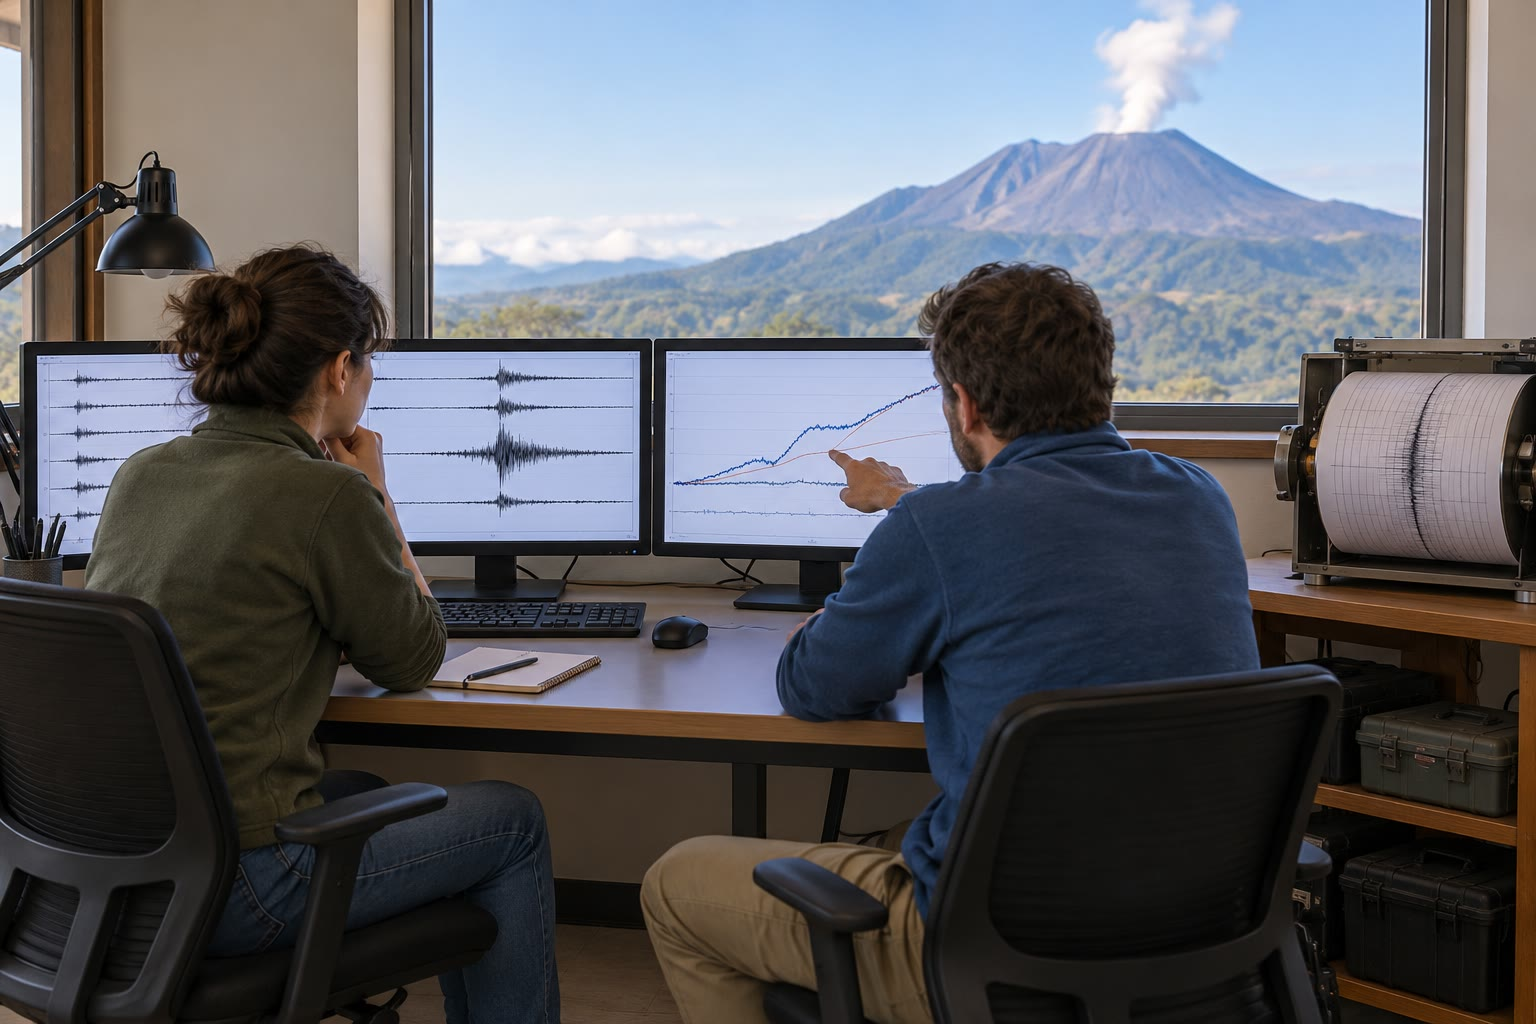
\includegraphics[width=\linewidth]{images/book4/ai/b2-volcano-observatory.jpg}
\par\smallskip{\scriptsize Scientifiques examinant des enregistrements sismiques dans un observatoire
volcanologique (illustration générée par IA).}
\end{minipage}
\end{inthefield}
% ledger: hvo:alert-levels

\section{Exercices}

\begin{exercise}[$\star$]\label{exo:b2:eruptive-styles:1}
Donner le VEI indiqué par le seul volume apparent de \omterm{def:b2:eruptive-styles:tephra}{téphra} pour~: (a) les cendres du mont
Saint-Helens, le 18~mai~1980, \qty{1.3}{km^3}~; (b) le dépôt de chute de la couche~5 du Cotopaxi,
\qty{0.29}{km^3}~; (c) une petite éruption de \qty{2e6}{m^3}. (d) Le matériau
éjecté par le Pinatubo en 1991 est donné comme «~plus de \qty{5}{km^3}~», pourtant
l'éruption est classée VEI~6. Quel volume apparent cette classification implique-t-elle au minimum~?
\end{exercise}
% ledger: usgs:vei-criteria, usgs:msh-1980-ash, biass19:layer5, usgs:pinatubo-1991

\begin{exercise}[$\star$]\label{exo:b2:eruptive-styles:2}
Nommer chaque \omterm{def:b2:eruptive-styles:tephra}{pyroclaste}~: (a) un éclat de verre long de \qty{0.5}{mm}~; (b) un
fragment de ponce large de \qty{3}{cm}~; (c) un morceau anguleux de vieille lave large de \qty{20}{cm}~;
(d) un grumeau fusiforme long de \qty{8}{cm}, aux extrémités tordues.
\end{exercise}
% ledger: nps:pyroclast-sizes

\begin{exercise}[$\star$]\label{exo:b2:eruptive-styles:3}
Avec $H = 0.304\,Q^{0.241}$ ($H$ en kilomètres au-dessus de l'évent, $Q$ en
\unit{kg/s})~: (a) calculer $H$ pour $Q = \qty{e6}{kg/s}$ et \qty{e8}{kg/s}~;
(b) calculer le débit massique impliqué par une colonne haute de \qty{35}{km}, et son
intensité $I = \log_{10}Q + 3$~; (c) indiquer de quel facteur varie $Q$ si la hauteur mesurée
est surestimée de \qty{20}{\percent}.
\end{exercise}
% ledger: aubry23:fits, brown14:record

\begin{exercise}[$\star$]\label{exo:b2:eruptive-styles:4}
Le dépôt de chute de la couche~5 du Cotopaxi a un volume apparent de \qty{0.29}{km^3}. En prenant une
masse volumique apparente de \qty{1000}{kg/m^3} pour le dépôt et \qty{2500}{kg/m^3} pour le
\omterm{def:b2:magma-emplacement:magma}{magma}, calculer son volume d'équivalent roche dense, sa masse et sa magnitude
$M = \log_{10}m - 7$.
\end{exercise}
% ledger: biass19:layer5, brown14:record

\begin{exercise}[$\star\star$]\label{exo:b2:eruptive-styles:5}
Un dépôt de chute a une épaisseur de \qty{40}{cm} sur l'isopaque de $\sqrt A = \qty{5}{km}$
et de \qty{10}{cm} sur celui de $\sqrt A = \qty{15}{km}$, et il s'amincit selon une seule
exponentielle. Calculer $k$, $T_0$, la demi-distance d'épaisseur $\ln 2/k$, le volume
apparent et le VEI.
\end{exercise}

\begin{exercise}[$\star\star$]\label{exo:b2:eruptive-styles:6}
(a) Établir que le volume à l'intérieur de l'isopaque $x = \sqrt A$ d'un dépôt qui s'amincit
comme $T_0e^{-kx}$ vaut $\frac{2T_0}{k^2}[1 - (1 + kx)e^{-kx}]$. (b) Résoudre $(1 + u)e^{-u} =
1/2$ à trois chiffres significatifs près, par substitutions successives ou par dichotomie. (c) Pour
le dépôt de l'\cref{exo:b2:eruptive-styles:5}, au-delà de quel isopaque se trouve la moitié du volume~? Comparer
avec la distance à l'évent de l'isopaque le plus éloigné ayant été cartographié.
\end{exercise}

\begin{exercise}[$\star\star$]\label{exo:b2:eruptive-styles:7}
Un \omterm{def:b2:magma-emplacement:magma}{magma} rhyolitique à \qty{850}{\celsius} (\qty{1123}{K}) contient
\qty{5.0}{\percent} d'eau, avec une solubilité $s = 0.444$ pour cent par
$\sqrt{\unit{MPa}}$~; sa masse volumique est de \qty{2300}{kg/m^3}. (a) Calculer sa
\omterm{def:b2:magma-emplacement:volatiles}{pression de saturation en volatils}, et la profondeur à laquelle elle est atteinte pour un
gradient de pression de \qty{0.025}{MPa/m}. (b) Calculer la fraction volumique de gaz à
\qty{10}{MPa} si le gaz reste dans le \omterm{def:b2:magma-emplacement:magma}{magma} ($R = \qty{8.314}{J/(mol.K)}$, $M =
\qty{0.018015}{kg/mol}$). (c) Expliquer pourquoi les \omterm{def:b2:magma-emplacement:magma}{magmas} basaltiques se fragmentent bien moins
souvent, alors qu'à \qty{1}{MPa} un basalte en système fermé, à \qty{1}{\percent} d'eau, serait
constitué à \qty{92}{\percent} de gaz~?
\end{exercise}
% ledger: moore98:h2o, cassidy18:fragmentation, cassidy18:ascent

\begin{exercise}[$\star\star$]\label{exo:b2:eruptive-styles:8}
(a) Une \omterm{prop:b2:eruptive-styles:mogi}{source de Mogi} située à \qty{5}{km} de profondeur gagne \qty{e7}{m^3}. Calculer le
soulèvement au-dessus d'elle ($\nu = 0.25$). (b) Un autre renflement tombe à la moitié de son maximum à
\qty{3.8}{km} de son centre~: déterminer la profondeur de sa source. (c) Calculer la fraction du
soulèvement maximal qu'une station observe à une distance horizontale égale à la profondeur
de la source.
\end{exercise}
% ledger: dmodels:mogi

\begin{exercise}[$\star\star$]\label{exo:b2:eruptive-styles:9}
Une explosion vulcanienne projette des blocs hors d'un cratère. En négligeant la résistance de l'air
et la hauteur du bord du cratère, calculer la portée maximale d'un bloc lancé à \qty{100}{m/s},
puis à \qty{200}{m/s} ($g = \qty{9.81}{m/s^2}$). La résistance de l'air donne-t-elle une borne
supérieure ou inférieure à ces portées~? Expliquer pourquoi une zone de danger balistique
autour d'un évent croît comme le carré de la vitesse de lancement.
\end{exercise}

\begin{exercise}[$\star\star\star$]\label{exo:b2:eruptive-styles:10}
(a) Établir le volume d'un dépôt à deux segments exponentiels donné dans l'encadré Méthode,
en supposant l'épaisseur continue au point de croisement des droites. (b) Pour
la couche~5 du Cotopaxi, les segments ajustés sont $T = \qty{1285}{cm}\times
e^{-0.365x}$ et un segment distal de pente $k_2 = \qty{0.138}{km^{-1}}$, qui se croisent en
$X = \qty{8.56}{km}$. Calculer le volume et la part de celui-ci au-delà du
point de croisement.
\end{exercise}
% ledger: biass19:layer5

\begin{exercise}[$\star\star\star$]\label{exo:b2:eruptive-styles:11}
(a) En utilisant la \cref{prop:b2:eruptive-styles:plume}, indiquer de quel facteur croît la hauteur d'une
colonne lorsque le débit d'éruption est multiplié par 100. Comparer avec les exposants empiriques $0.241$ et
$0.226$. (b) Dire de quelle façon une atmosphère plus fortement stratifiée modifie la hauteur, et de combien
si $N$ croît de \qty{20}{\percent}. (c) Donner deux raisons pour lesquelles les exposants mesurés
peuvent être inférieurs
à $1/4$.
\end{exercise}
% ledger: aubry23:fits

\begin{exercise}[$\star\star\star$]\label{exo:b2:eruptive-styles:12}
Le catalogue mondial recense 132 éruptions de VEI~4 ou plus survenues entre 1500
et 1899, et 95 entre 1900 et 2024. (a) Calculer le taux par siècle dans chaque
période. (b) Si le taux depuis 1900 est le taux réel, quelle fraction des éruptions anciennes a été
consignée~? (c) Une étude des grandes éruptions compte 21 éruptions de magnitude 4 à 4.9 par siècle
entre 1500 et 1900, et 56 depuis 1900~; comparer. (d) Expliquer pourquoi cette fraction
dépend de la taille des éruptions.
\end{exercise}
% ledger: data:b4-gvp-eruptions, brown14:record

\section{Problème~: lecture d'un dépôt plinien}

\begin{problem}[{Problème du week-end --- à partir des isopaques d'une chute de ponce jusqu'à la taille
de son éruption, de la hauteur de sa colonne et de la fréquence de ces
éruptions}]
\label{pb:b2:eruptive-styles:1}
Un volcan imaginaire a laissé une chute de ponce issue d'une seule phase plinienne d'une durée de
\num{10}~heures. Une fois l'allongement dû au vent retiré en utilisant la racine carrée de leurs aires,
ses isopaques sont~:
\begin{center}
\small
\begin{tabular}{lccccc}
\hline
$\sqrt A$ (\unit{km}) & 10 & 20 & 40 & 80 & 120 \\
épaisseur $T$ (\unit{cm}) & 200 & 100 & 48 & 14 & 4.0 \\
\hline
\end{tabular}
\end{center}
Données~: masse volumique apparente du dépôt \qty{900}{kg/m^3}~; masse volumique du
\omterm{def:b2:magma-emplacement:magma}{magma} \qty{2400}{kg/m^3}~; hauteur de la colonne mesurée sur les plus gros fragments,
\qty{31}{km} au-dessus de l'évent~; tropopause à \qty{16}{km}. Utiliser $H =
0.304\,Q^{0.241}$ et $H = 0.345\,Q^{0.226}$ ($H$ en kilomètres, $Q$ en
\unit{kg/s}).

\medskip\noindent\textbf{Partie I --- Le dépôt.}
\begin{enumerate}
\item Calculer $\ln T$ pour chaque isopaque et montrer que les points se répartissent sur deux
segments droits lorsqu'on les porte en fonction de $\sqrt A$. Où se trouve la rupture~?
\item Calculer la pente $k_1$ et l'ordonnée à l'origine $T_0$ du segment proximal passant par les
deux premières isopaques.
\item La droite des moindres carrés passant par les trois isopaques distaux est $T =
\qty{167}{cm}\times e^{-0.0311\sqrt A}$. Vérifier qu'elle passe à moins de
\qty{5}{\percent} de chacun d'eux.
\item Calculer la valeur de $\sqrt A$ à laquelle les deux droites se croisent.
\item Calculer les demi-distances d'épaisseur $\ln 2/k$ des deux segments.
\item Calculer le volume que le dépôt aurait s'il s'amincissait partout selon la pente
proximale.
\item Calculer le volume apparent avec les deux segments, et la part apportée par la correction
du segment distal, moins pentu.
\item De quel facteur le volume serait-il sous-estimé si seul le dépôt proximal avait été cartographié~?
Pourquoi est-ce un risque réel pour les vieux dépôts~?
\end{enumerate}

\noindent\textbf{Partie II --- La taille de l'éruption.}
\begin{enumerate}[resume]
\item Donner le VEI de l'éruption.
\item Calculer le volume d'équivalent roche dense.
\item Calculer la masse émise.
\item Calculer la magnitude $M = \log_{10}m - 7$.
\item Combien de fois ce dépôt est-il plus grand que la chute de cendres du mont
Saint-Helens en 1980, \qty{1.3}{km^3}~?
\item Quelle hauteur de colonne le tableau des VEI associe-t-il à cette éruption, et quel
style~?
\end{enumerate}

\noindent\textbf{Partie III --- La colonne.}
\begin{enumerate}[resume]
\item Calculer le débit massique moyen sur toute la phase plinienne, et son
intensité $I = \log_{10}Q + 3$.
\item Calculer la hauteur de colonne prédite par la première loi empirique.
\item Même calcul avec la seconde loi.
\item Comparer avec les \qty{31}{km} mesurés sur les fragments, compte tenu de la dispersion
des lois.
\item Quel débit massique impliquerait \qty{31}{km} selon la première loi~? De quel facteur
diffère-t-il de celui de la question~15, et qu'est-ce qui pourrait l'expliquer~?
\item La colonne a-t-elle injecté du gaz dans la stratosphère~? Quelles en seraient les conséquences
pour le climat, et quel serait le gaz clé~?
\end{enumerate}

\noindent\textbf{Partie IV --- À quelle fréquence~?}
\begin{enumerate}[resume]
\item À partir des décomptes du catalogue (399 éruptions de VEI $\ge 3$ de 1950 à
2024, 95 de VEI $\ge 4$ depuis 1900, 22 de VEI $\ge 5$ depuis 1800, 8 de VEI $\ge 6$ depuis
1500, toutes fenêtres se terminant en 2024 incluse), calculer les quatre taux annuels et
leurs logarithmes.
\item Vérifier que la droite $\log_{10}\lambda_v = 3.28 - 0.85\,v$ passe à moins de
\qty{10}{\percent} de chaque taux.
\item Pourquoi chaque fenêtre commence-t-elle plus loin dans le passé pour les éruptions plus grandes~?
\item À partir de la droite, calculer le taux des éruptions de VEI $\ge 5$, leur
période de retour moyenne, et la probabilité d'en avoir au moins une dans les dix prochaines années.
\item À partir de la droite, calculer le taux des éruptions de VEI $\ge 7$ et le comparer
aux deux survenues depuis l'an 1000.
\item À partir de la droite, calculer le taux des éruptions de VEI $\ge 6$ et la
probabilité, en pour cent, d'en avoir au moins une n'importe où sur Terre dans les 100
prochaines années, chiffre clé de ce problème. Sur quelle hypothèse repose-t-elle~?
\end{enumerate}
\end{problem}
